\documentclass{llncs}
\usepackage{graphicx}
\usepackage{url}
\usepackage{amsmath}

\begin{document}
\title{Proiect verificare formală}
\author{Arpad Precup \inst{1}, Elber Da \inst{2}, Szopuch Denis \inst{3} Radu Bogdan \inst{4}}
\institute{
    Universitatea de Vest din Timișoara,\\
  Inginerie Software\\
    \email{} 
}

\maketitle
\newpage

\section{Abstract}
Acest proiect explorează procesul de instalare și rulare al MiniSat, un solver SAT de înaltă performanță, pe sisteme de operare variate, cu un focus specific pe Windows 10, Linux și pe o mașină virtuală cu Ubuntu. Problema SAT (satisfiabilitatea formulelor logice) este una dintre cele mai importante în informatică, având numeroase aplicații în domenii precum verificarea formală, inteligența artificială și teoria complexității. Proiectul documentează pașii de instalare și configurare a MiniSat, provocările întâmpinate în setările de debugging și compilare, precum și soluțiile aplicate pentru a obține o rulare funcțională a aplicației în medii de dezvoltare diferite.

\keywords{MiniSat · SAT Solver · Instalare · Debugging ·}

\section{Introducere}

Problema satisfiabilității, cunoscută sub acronimul SAT, este o problemă esențială în teoria complexității computaționale, fiind prima problemă demonstrată ca fiind NP-completă. Aceasta constă în determinarea unei atriburi de adevăr pentru variabilele unei expresii logice astfel încât întreaga expresie să fie satisfăcută. Soluționarea problemelor SAT a devenit fundamentală într-o varietate de aplicații, inclusiv verificarea formală a software-ului și hardware-ului, inteligența artificială, optimizarea și bioinformatica.

MiniSat este un solver SAT de înaltă performanță, dezvoltat pentru a participa în competițiile SAT și pentru a rezolva probleme complexe de satisfiabilitate. MiniSat utilizează algoritmi avansați, precum DPLL (Davis-Putnam-Logemann-Loveland) și CDCL (Conflict-Driven Clause Learning), pentru a explora eficient spațiul de căutare al soluțiilor posibile. Datorită eficienței sale și accesibilității ca proiect open-source, MiniSat este adesea utilizat ca reper în benchmark-urile SAT și este o alegere populară pentru studii și cercetări în domeniul satisfiabilității.

Acest proiect urmărește să documenteze procesul de instalare și configurare a MiniSat pe diverse platforme, punând accent pe provocările întâmpinate pe Windows și Linux, inclusiv rularea în mod debugging. De asemenea, include soluții pentru configurarea mediului de dezvoltare Visual Studio Code (VSCode), astfel încât să permită rularea și testarea programului într-un mod flexibil și reproductibil. Această lucrare va contribui la îmbunătățirea accesului la documentație pentru dezvoltatori și cercetători interesați de utilizarea MiniSat pe platforme multiple.

\newpage

\section{Descrierea Problemei SAT}

Problema satisfiabilității, cunoscută sub numele de SAT, constă în determinarea valorilor de adevăr pentru variabilele unei expresii logice astfel încât întreaga expresie să fie satisfăcută, adică evaluată ca adevărată. În limbajul logicii propoziționale, o expresie este satisfiabilă dacă există o atribuire a valorilor variabilelor sale care face întreaga expresie să fie adevărată. Această problemă are o importanță majoră în teoria complexității deoarece este prima problemă cunoscută ca fiind NP-completă, fiind astfel esențială în clasificarea și înțelegerea problemelor computaționale complexe.

Algoritmii utilizați pentru rezolvarea problemelor SAT includ tehnici diverse, cei mai reprezentativi fiind algoritmul DPLL și tehnica CDCL. Algoritmul DPLL (Davis-Putnam-Logemann-Loveland) utilizează tehnici de căutare recursivă, reducând treptat problema prin atribuiri succesive ale variabilelor și eliminarea condițiilor imposibile. CDCL (Conflict-Driven Clause Learning) este o optimizare a DPLL, care învață din conflictele întâlnite în timpul căutării soluției, reducând astfel numărul de căi explorate.

Aplicațiile problemelor SAT sunt vaste și acoperă domenii variate, de la verificarea formală a corectitudinii sistemelor software și hardware până la inteligența artificială și bioinformatică. MiniSat, fiind un solver SAT foarte eficient, este utilizat adesea pentru a testa diverse benchmark-uri SAT și pentru a valida probleme complexe în cercetare și dezvoltare.



\section{Instalare MiniSat}

\subsection{Instalare pe Windows 10}

Pentru a instala MiniSat pe Windows 10, urmăm câțiva pași ce implică descărcarea codului sursă și configurarea unui mediu de dezvoltare compatibil. MiniSat este un proiect scris în C++, astfel că vom folosi Visual Studio Code sau un IDE similar pentru a permite compilarea și rularea codului C++. Este necesară instalarea MinGW, o suită de unelte care aduce funcționalitățile GNU Compiler Collection (GCC) pe Windows. 

1. Descărcăm codul sursă MiniSat de pe GitHub-ul oficial al proiectului.
2. Instalăm MinGW pentru a putea compila codul C++.
3. Configurăm mediul de lucru în VSCode și adăugăm un fișier `launch.json` pentru a permite rularea în modul debugging.
4. În timpul instalării am întâmpinat erori legate de tipizare strictă; astfel, a fost necesar să folosim opțiunea `CXXFLAGS="-fpermissive"` pentru a ignora aceste erori și a permite compilarea.


\subsection{Instalare pe Linux}

Instalarea MiniSat pe un sistem Linux este relativ simplă, datorită accesibilității librăriilor necesare și a suportului nativ pentru GNU Compiler Collection (GCC). Procesul se realizează prin terminal și implică actualizarea sistemului, descărcarea codului sursă, compilarea și rularea acestuia.

1. Actualizăm lista de pachete și instalăm dependențele necesare.
2. Descărcăm și compilăm codul MiniSat din repo-ul oficial.
3. Pentru rularea cu succes a compilării a fost necesară utilizarea `CXXFLAGS="-fpermissive"`, fără de care procesul întâmpina erori de tipizare strictă.
4. Configurăm un fișier `launch.json` pentru rularea în VSCode, care facilitează debugging-ul și rularea aplicării MiniSat într-un mod ușor de gestionat.


\subsection{Instalare pe o Mașină Virtuală cu Ubuntu}

După ce Ubuntu este instalat pe mașina virtuală, deschidem terminalul și actualizăm pachetele sistemului cu comanda:
"sudo apt update \&\& sudo apt upgrade"
Apoi, instalăm dependențele necesare pentru compilare:
"sudo apt install g++ make git"
Clonăm codul sursă al MiniSat de pe GitHub:
"git clone https://github.com/niklasso/minisat.git"
Accesăm directorul minisat:
"cd minisat"
Și compilăm MiniSat folosind:
"sudo make CXXFLAGS="-fpermissive""
După finalizare, verificăm instalarea rulând:
"./minisat"


\section{Provocări Întâmpinate}

\subsection{Instalarea pe Windows}

Instalarea MiniSat pe Windows a întâmpinat mai multe provocări, în special din cauza diferențelor dintre compilatorul Windows și cerințele stricte de tipizare din codul sursă al MiniSat. Am utilizat flag-ul `-fpermissive` pentru a permite compilatorului să ignore aceste diferențe și să accepte codul.

\subsection{Rularea în Mod Debugging}

Pentru a permite debugging-ul, a fost necesară setarea opțiunii `CXXFLAGS = -fpermissive -g -O0`. Aceste opțiuni au permis intervenții de depanare detaliată, iar MiniSat ar fi generat erori fără aceste flag-uri. Aceasta a făcut debugging-ul posibil pe Windows și Linux.

\subsection{Crearea fișierului launch.json în VSCode}

Pentru rularea MiniSat în Visual Studio Code, a fost necesară configurarea unui fișier `launch.json` specific, astfel încât MiniSat să fie accesibil prin extensia de C++ debugging din VSCode, oferind suport pentru testare și analiză interactivă.

\section{Benchmarks}
de unde au fost luate benchmarkurile (competitia SAT 2024) + familia aleasa (clique coloring) + pe ce masini au rulat testele + rezultatele (tabelele) + observatii

\section{Codul Minisat}
MiniSat este un SAT solver disponibil public sub formă de repository pe GitHub (TODO adaugă link spre repo). A fost creat cu scopul de a ajuta la introducerea de noi membrii în comunitatea SAT prin furnizarea unui SAT solver de dimensiuni reduse (dar eficient) și documentat (TODO adaugă biografie din http://minisat.se/MiniSat.html). Cu toate că are dimensiuni reduse, MiniSat este un SAT solver complet și, cel puțin pentru data apariției sale în 2003, suportă toate funcționalitățile de ultimă oră are solverelor, precum: învățare bazată pe conflicte, backtracking bazat pe conflicte și two-literal watch scheme.

\subsection{Structura fizică}
Proiectul MiniSat are următoare structură:
\begin{enumerate}
    \item \texttt{minisat/mtl/} - reprezintă Mini Template Library-ul asociat MiniSat. Conține diferite structuri de date generice care fac posibilă utilizarea MiniSat fără nevoia altor dependințe. În acest directory se găsesc, spre exemplu, implementări pentru structuri de date precum: Maps, cozi și vectori.
    \item \texttt{minisat/utils/} - conține helpere pentru cod. Spre exemplu, aici se găsesc metodele folosite pentru a interacționa cu sistemul I/O al mașinii pe care MiniSat este rulat și metode generice de parsat text: trecerea peste spațiile albe, trecerea peste o linie.
    \item \texttt{minisat/core/} - Versiunea core a MiniSat. Cu ajutorul metodelor și structurilor de date prezente în fișierele anterior menționate, aici are loc procesul de SAT solving. Aceasta este versiunea asupra căreia ne-am concentrat atenția.
    \begin{enumerate}
        \item \texttt{Dimacs.h} - Un fișier de tip header, care conține trei metode: \textbf{parse\_DIMACS}, \textbf{parse\_DIMACS\_main} și \textbf{readClause}. Dintre acestea, doar metoda \textbf{parse\_DIMACS} este apelată din exteriorul acestui fișier, aceasta fiind apelată din Main.cc pentru a insera problema (care este reprezentată într-un fișier text al cărui conținut trebuie să respecte formatul DIMACS) în Solver.
        \item \texttt{Main.cc} - Punctul de intrare în program. Acesta acceptă diferiți parametrii care pot fi utilizați pentru a particulariza execuția codului. Spre exemplu, prin folosirea parametrului \textbf{"verb"} pot fi selectate trei nivele de verbozitate, care modifică numărul de log-uri afișate pe parcursul rulării programului. Alți parametrii care pot fi setați: limită de timp pentru rulare (folosind parametrul \textbf{"cpu\_lim\"}), limită memorie folosită (folosind parametrul \textbf{"mem\_lim"}).
        \item \texttt{Solver.cc} - Conține codul pentru Solver. Conține metode care crează noi variabile, adaugă cluaze, rezolvă problema. Conține de asemenea și diferiți membrii precum modelul, acesta reprezentând o soluție, dacă aceasta a fost găsită.
        \item \texttt{Solver.h} - header-ul pentru clasa Solver.
        \item \texttt{SolverTypes.h} - Fișier header care conține definiția mai multor tipuri de date folosite pentru Solver, printre care clasa \textbf{Clause} și struct-ul \textbf{Lit}. Este prezentat mai pe larg ce reprezintă aceste structuri de date în capitolul (TODO adauga link care sa duca la sectiunea structuri de date).
    \end{enumerate}
    \item \texttt{minisat/simp/} - Un solver extins care are capabilități pentru aplicarea de simplificări, fapt care ajută la o performață mai bună. 
\end{enumerate}

\subsection{Structura arhitecturală}
% Prezinta high level care sunt componentele principale ale SAT solver (adauga diagrama UML?)
Componenta principală arhitecturală o reprezintă clasa \textbf{Solver}. Odată inserată problema în solver (folosind metoda \textbf{parse\_DIMACS}), acesta este capabil de a o rezolva prin intermediul metodei \textbf{solve\_}. Informații amănunțite despre cum funcționează metoda \textbf{solve\_} sunt disponibile în secțiunea (TODO adaugă link la flow-uri impoprtante).

La nivel de diagramă de secvență, fluxul de date de la rulare la afișarea output-ului este următorul:

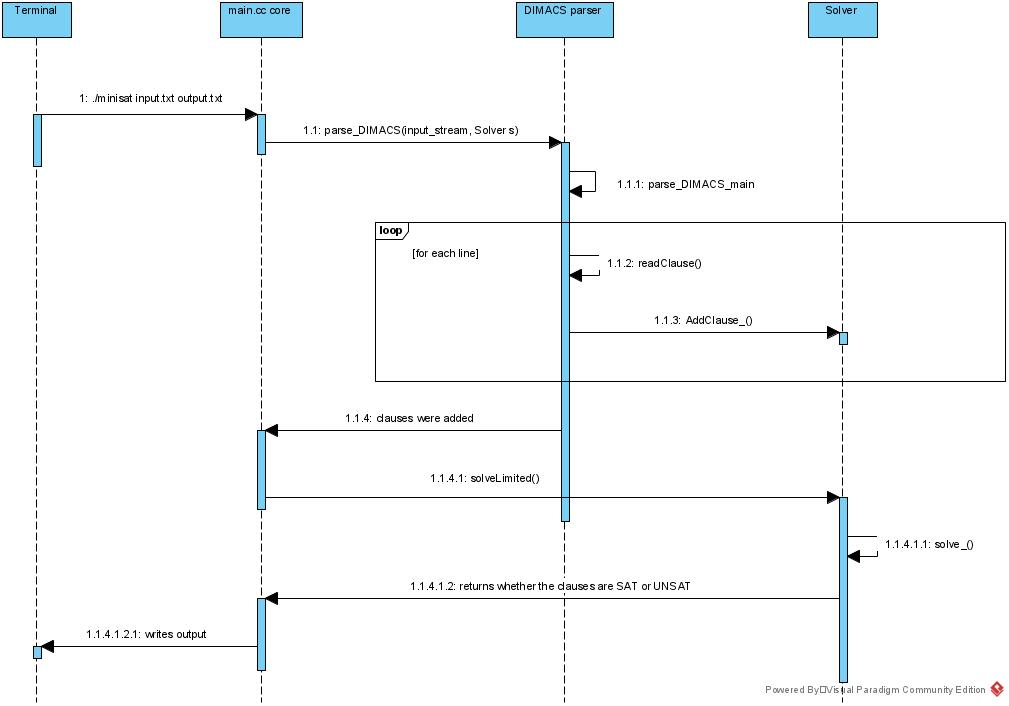
\includegraphics[width=0.8\textwidth]{resources/Minisat_main_sequence_diagram.jpg}

\subsection{Structuri de date}
% Prezinta cateva dintre structurile de date folosite si cum sunt folosite: ex. Lit
Datorită naturii problemei abordate de MiniSat, au fost declarate mai multe tipuri speciale de structuri de date peste care vom trece în această secțiune.
\begin{itemize}
    \item \textbf{Var} - este o definiție de tip care este defapt un simplu integer. Variabilele trebuie alese de la 0 la N pentru a putea fi folosite ca indecși în vectori. Totodată, se declară și o instanță specială de tipul \textbf{Var} care reprezintă o variabilă neasignată, care are valoare -1. Aceste variabile reprezintă fiecare literal parsat din fișierul de input, cu o mică ajustare: \textbf{Var}, fiind folosite ca indecși de vectori nu pot avea valori negative. De asemenea, trebuie să înceapă de la valoarea 0. Având în vedere că în formatul DIMACS literalii încep de la valoare absolută 1, valoare \textbf{Var} asociată se calculează prin decrementarea valoarii absolute a literalului. Astfel, spre exemplu, dacă literalul parsat este "-1", valoare \textbf{Var} asociată este 0.
    \item \textbf{Lit} - este un struct care conținând o singură valoare de tip integer este capabil să encodeze un literal cu tot cu semnul asociat, folosindu-se de semnul literalului parsat și de valoarea \textbf{Var} asociată acestuia. Acest lucru este făcut posibil prin modul ingenios prin care valoarea din struct-ul \textbf{Lit} este calculată. Aceasta este calculată ca fiind dublul valorii \textbf{Var} asociate la care se adaugă 1 daca semnul literalului este negativ. Astfel, fiecărei posibile variabile \textbf{Var} îi sunt asociate două valori: 2 * var sau 2 * var + 1 (dacă semnul literalului este negativ).
    
    Așadar se ajunge ca int-ul stocat în \textbf{Lit} să aibă encodat pe cel mai puțin semnificant bit valoare semnului, iar pe restul de biți valoare \textbf{Var} de la care provine. Exemplu: Daca literalul parsat este -7, atunci \textbf{Var}-ul asociat este 6. Luând în considerare și semnul literalului, variabila stocată în \textbf{Lit} va fi 13 (6 * 2 + 1). în reprezentare binară 13 este 1101, ultimul bit (1) reprezentând faptul că literalul este negat, iar restul reprezentând valoare \textbf{Var} asociată 0b110 = 6
    \item \textbf{Clause} - este o clasă care reprezintă o clauză. Conține un vector de \textbf{Lit} și diferite câmpuri care stochează date despre clauză cum ar fi dacă a fost învățată sau dimensiunea acesteia.
    \item \textbf{VMap} - o structură de date folosită în multe câmpuri din clasa Solver pentru a stoca date de tip cheie -> valoare, unde cheia este de tip \textbf{Var}. Exemple de astfel de câmpuri în solver sunt: \textbf{assigns} (stochează asignările curente pentru fiecare variabilă) și \textbf{polarity} (stochează polaritatea preferată pentru fiecare variabilă).    
\end{itemize}
\subsection{Metode remarcabile}
% Prezinta functii importante din code (ex. metoda search, unit propagation etc.)
În această secțiune sunt prezentate câteva dintre metodele importante folosite pentru a rezolva problema satisfiabilității în MiniSat.
\subsubsection{Solve} - Metoda care implementează strategia de rezolvarea a problemei la nivelul cel mai superior. Această metoda folosește metoda \textbf{Search} și o restartează până când se ajunge la o concluzie sau "bugetul" (numărul de conflicte și propagări permise) este depășit. În repository-ul de GitHub al echipei noastre se poate vedea diagrama de activitate asociată acestei metode (TODO insert link).
\subsubsection{Search} - cea mai complexă procedură. În această procedură, variabilele sunt alese și le sunt atribuite valori (aceste asignări sunt stocate într-un vector de \textbf{Lit} numit \textbf{trail}. De asemenea, într-un vector de integers numit \textbf{trail\_lim} se rețin indecșii de la care încep nivele diferite de decizie în \textbf{trail}), până în momentul în care propagarea determină un conflict, punct în care se creează o clauză conflict care este adăugată Solver-ului ca și clauză învățată. Apoi se face backtracking, anulând asignările făcute la nivele mai înalte decât nivelul de la care a pornit conflictul (folosind informațiile din \textbf{trail} și \textbf{trail\_lim}. Odată procesul de backtracking terminat, se reîncepe cu procesul de propagare.

\begin{figure}[h]
\centering
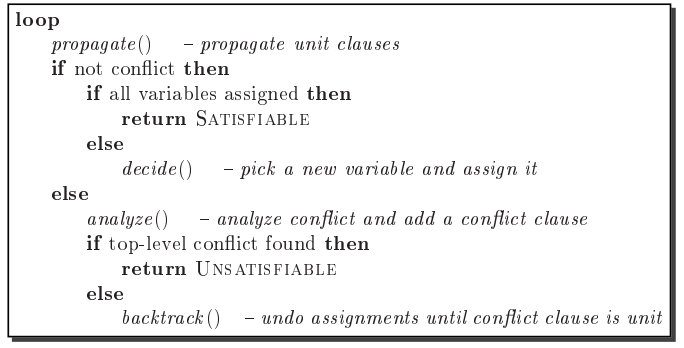
\includegraphics[width=0.8\textwidth]{resources/search_pseudocode.png}
\caption{Pseudocod pentru metoda \textbf{Search}. Sursă TODO. De asemenea, diagrama de activitate poate fi găsită în proiectul echipei noastre de GitHub TODO link}
\end{figure}

\subsubsection{Propagate} - Metoda care se ocupă de propagarea unității. 80\% din timpul de rulare MiniSat este datorat propagării, astfel această metodă poate fi considerată principală țintă când se dorește îmbunătățirea performanței (TODO source). Această metoda folosește two-literal watch scheme pentru a eficientiza propagarea unitară. Diagramă de activitate poate fi găsită pe GitHub-ul asociat proiectului nostru (TODO add link).


\section{Propriul nostru repository si cum am impartit task-urile}

\section{Concluzii}

Acest proiect a demonstrat cum MiniSat poate fi instalat și utilizat pe platforme diferite, inclusiv Windows, Linux și Ubuntu. Provocările întâmpinate au fost legate de erorile de compilare și setările de debugging, dar soluțiile aplicate au permis obținerea unui mediu de dezvoltare stabil și eficient.

\end{document}